\documentclass[man,noapacite]{apa2} 

\usepackage{apacite2}
\usepackage{amssymb}
\usepackage{graphicx}

\title{Using Tablets to Collect Data from Young Children} 

\author{Michael C. Frank, Elise Sugarman, Alexandra Horowitz, \\ Molly L. Lewis, \& Daniel Yurovsky} 

\affiliation{Department of Psychology, Stanford University}

\abstract{Mobile, touch-screen devices are increasingly ubiquitous in children's lives. The extensive use of such devices provides both a challenge and an opportunity for developmental psychologists. While more research is needed to understand the nature and consequences of young children's interaction with such devices, they nevertheless present an exciting opportunity for data collection. We describe a simple method for creating cross-platform, interactive tablet experiments using open web-based resources. We illustrate this method by collecting data from children 1--5 years old in a simple word-recognition paradigm and show that it yields reliable accuracy and reaction time data; we provide code for this experiment for the use of other researchers. Tablets should hence be considered as a viable method for collecting low-cost, well-controlled developmental data.}

\shorttitle{Tablet-based Data Collection} 
\rightheader{TABLET-BASED DATA COLLECTION}

\acknowledgements{We gratefully acknowledge the families and staff at San Jose Children's Discovery Museum and the laboratory of Anne Fernald for sharing their visual stimuli. An earlier version of this material was previously presented in a blogpost \cite{frankblogpost}. Thanks to Janelle Klaas, Andrew Weaver, and Sarah James for assistance in data collection. Please address all correspondence to Michael C. Frank, Department of Psychology, Jordan Hall (Bldg. 420), 450 Serra Mall, Stanford, CA 94305. Phone: (650) 724-4003. E-mail: \texttt{mcfrank@stanford.edu}}

\begin{document}

\maketitle

%\setlength{\textfloatsep}{0.02cm}

\section{Introduction}

Since Apple debuted the iPad in 2010, the ubiquity of personal tablets---interactive, touchscreen-based computing devices, typically larger than a phone but smaller than a laptop---has skyrocketed. By 2013, an estimated 75\% of families with young children in the United States owned a mobile device, with 40\% of households owning tablets \cite<20\% of lower-income families and 63\% of higher-income families;>{rideout2014}; tablets were estimated to constitute 19\% of children's overall screen time from ages 0--8. Accordingly, the market for downloadable applications targeted to children has increased dramatically, representing 72\% of the top selling apps in the iTunes store, and over 80\% in the Education category \cite{shuler2012},  although one report suggests the viewing photos is the most popular activity for children under age 4 \cite{cristiainpress}. This explosion in popularity has created a surge of interest in both the consequences of tablet use for children and the potential for using these devices as scientific tools. 

Nevertheless, there are significant challenges involved in using tablets for research. These include the difficulty and potential costliness of developing custom applications (``apps'') for individual experiments, technical problems with app distribution and cross-device compatibility, and the lack of data confirming the reliability of data collected with tablets. Perhaps for these reasons, there is currently a paucity of published articles that use tablets to collect developmental data. 

The goal of the current article is to address these challenges. We begin by briefly reviewing research on the use of tablets in children. We then describe a method for using standard, freely-available web-development tools to create tablet-based experiments. Although this method requires some programming experience, it is significantly easier than developing tablet-native applications and has relatively few drawbacks from the research perspective. We next show how this method can be used to implement a simple word-recognition experiment. Our data suggest that the tablet platform is an engaging method for data collection that yields reliable accuracy and reaction time from young children. 

\section{Prior Work on Children's Tablet Use}

The primary focus of research on tablets with children has been evaluation of their educational potential. We briefly review this literature and then turn to the issue of characterizing children's interactions. The starting point for investigations of learning from tablets is the suggestion that children learn less from passive video viewing than they do from live demonstrations, a phenomenon known as the video deficit effect \cite<e.g.>{anderson2005,deloache2010,kuhl2003}. These findings influenced the American Academy of Pediatrics (AAP) to uphold a policy recommending no ``screen time'' for children under age 2 \cite{brown2011}.

% A survey of parent reports of television-viewing and children's vocabulary under age 2 found that infants who spent more time viewing infant-directed programs (``baby media,'' such as the Baby Einstein series), had lower vocabulary (\citeNP{zimmerman2007}; but see \citeNP{ferguson2014} for a recent reevaluation of these data). 

The experiences offered by touch-screen devices may be distinct from passive viewing of television and computer screens, however. \citeA{christakis2014} notes that the AAP's published media recommendation of no screen time was made before the release of tablet devices, and suggests that the policy should be revised to distinguish and accommodate some time with touch-screens. He proposes that tablets can offer a number of potential benefits that many traditional toys do not. Specifically, tablets are reactive (responding contingently to the child’s actions), interactive (eliciting responses from the child based on his or her actions), tailorable (modifiable according to age or preference), progressive (can increase in difficulty or complexity with experience), highly portable, and able to promote joint attention (a child and caregiver can interact with the program together).
% \footnote{Indeed, a joint statement by the National Association for the Education of Young Children and the Fred Rogers Center for Early Learning and Children's Media suggests that a single ``screen time'' recommendation oversimplifies the possible benefits of new technologies, and educators should explore the potential pros and cons of interactive medias to determine when and whether they are appropriate to support children's learning \cite{radich2013}.}
% Touch screens offer an interactive experience with feedback contingent on the child's touch; these devices have a range of features that can be individualized to a child's age and performance. 

While screens are not recommended as replacements for live interactions, interactive technologies may pose a number of benefits over other passively-viewed screen alternatives. Some work suggests that practice with interactive games may benefit attention and motor control \cite{bavelier2010}, and more generally screen time with tablets can promote independence, opportunities for physical closeness, and feelings of fun and accomplishment \citeA{rvachew2013}. The contingent feedback and individualization offered by mobile devices may thus make them a better medium for learning and engagement than traditional view-only screens. Such benefits may also make them valuable tools for research and evaluation.

In addition, young children do demonstrate some learning from interactive screen content, suggesting that ``video deficit'' effects may be limited to---or at least strongest in---passive viewing of pre-recorded material. In one study, \citeA{roseberry2014} found that 24- to 30-month-olds successfully learned a novel verb from a live interaction via video chat, while a yoked group who saw the same input with non-contingent presentation failed to learn.
% They taught 24- to 30-month-olds novel verbs in one of three conditions: in-person demonstration, video chat demonstration, or a yoked video demonstration (recorded from a different child, therefore not socially-contingent to the participant). They found that toddlers were able to learn the new verbs above chance and equally well for both of the socially-contingent conditions (in-person and video chat demonstrations), but were only at chance in the control condition. Even despite challenges from in-person information (e.g. skewed gaze cues due to the position of the camera), the contingent feedback appears to drive children’s ability to learn through live video interactions.
Young children also show some evidence of transferring learning between screens and physical objects. \citeA{zack2009} examined 15-month-olds' ability to transfer knowledge learned via a touch-screen or physical toy to another example either in the same presentation modality or across modalities. Children were most successful when toys were presented in the same modality, but children in the cross-modality conditions performed better than a no-demonstration baseline. Even before age 2, children thus show evidence of comprehending actions and goals presented on touch-screen devices and can transfer this knowledge between physical and 2-dimensional presentations.

One concern with children's performance is the accuracy of their motor control. Experience with tablets likely plays a substantial role in modulating the accuracy of children's interactions with tablets. \citeA{couse2010} found that young children could quickly learn to provide precise motor input on tablets with minimal training using a stylus pen. They had teachers rate the quality and complexity of 3- to 6-year-old's self-portraits created digitally on a tablet art program compared with their drawing using traditional writing tools on paper. Children were highly engaged with tablet program, their drawings were rated as typical or exceeding their typical quality of drawing, and three quarters of children on the tablet task exhibited no to little frustration during the task despite a number of technical challenges. Additionally, although researchers were prepared to give children up to four warm-up sessions using a stylus pen on tablet computer, most children advanced after a single warm-up phase. Altogether, these studies suggest that preschoolers and kindergarteners are highly motivated and competent at interacting with touch-screen tablets. 

And although children show interest and remarkable capabilities to use touch-screens even before they learn to talk, some affordances of mobile tablets are easier to master from young ages than others. \citeA{aziz2014} tested 2- to 5-year-olds in Malaysia and the United Kingdom on their ability to perform the seven most common touch gestures of iPads: tap, drag/slide, free rotate, drag and drop, pinch, spread, and flick. By age 2, children mastered the tap and drag/slide gestures, and by age 3, they could reliably produce all by the spread gesture. By age 4, all children performed all of the gestures. \citeA{cristiainpress} additionally suggest that enabling multi-touch responding--allowing touches from more than one location to be recorded simultaneously--may reduce motor control issues of children trying to interact with the tablet while holding or resting their hand on other parts of the screen. 
% , and precision of touch input may be increased with tools such as fine-tipped stylus pens instead of finger touches.

In sum, research on tablets suggests that interactive media may provide more learning opportunities than passive viewing. Tablets are extremely engaging to children and may provide a valuable source of information, but designers of tablet materials for young children should take care to consider appropriate content and gesture capabilities for their target age group. 


\section{Why Collect Developmental Data With Tablets?}

% \subsection{The value of tablet-based data collection}

Researchers working with young children have access to a wide variety of experimental paradigms, ranging from behavioral forced-choice to eye-tracking and looking-time based measures \cite{aslin2007,gredeback2009}. Nevertheless, each of these methods has its drawbacks. Behavioral methods are flexible and easy to implement, but they can be subject to experimenter biases, and often require labor-intensive offline coding. In contrast, corneal-reflection eye-tracking methods are precise and unbiased, allowing tight experimental control, but can be expensive and are difficult to implement outside of tightly-controlled lab settings. In addition, eye-tracking paradigms are typically very limited in length as they tend to be non-interactive \cite<cf.>{deligianni2011}.

Tablet-based experimental paradigms can supplement both of these data collection modalities by allowing researchers to create engaging, interactive paradigms that are low cost but nevertheless offer some of the precision and experimental control of eye-tracking paradigms. In the sections below, we offer five reasons why tablets may be valuable tools for developmental research.

\subsubsection{Diverse measures} Tablets allow the collection of many different dependent variables, including forced-choice responding and gesture trajectories. We especially highlight the ability to measure reaction times using tablets. Reaction times provide a continuous, informative measure of cognitive process and have proven invaluable in both developmental \cite<e.g.>{fernald1998,marchman2008} and adult (e.g. \citeNP{sternberg1969} et seq.) studies. Behavioral paradigms that afford reaction time measurement for young children typically require time-consuming offline coding. In contrast, eye-tracking paradigms yield reaction times, but with the tradeoff that the paradigms typically have limited interactivity. 

\subsubsection{Engagement} Children across ages enjoy tablets and are highly motivated to explore new tablet-based tasks, allowing researchers to collect more data from individual children. As documented by  \citeA{couse2010} and many informal observations of infants' and young children's interest, the use of tablet-based devices may lead children to view tablet-based experiments as similar to engaging commercial apps. In addition, behavioral paradigms with young children often require a ``warm-up'' period so that the child is comfortable interacting with an unfamiliar experimenter; such a period can be shorter or absent to the extent that a tablet-based paradigm requires less face-to-face interaction. 

\subsubsection{Experimental control} Studies that involve interaction with an experimenter are the de-facto standard in cognitive development research, but such studies have as major drawbacks that it may be difficult or impossible to ensure that experimenters are blind to condition and hypothesis. Often hypotheses are simple enough that even ``na\"ive'' research assistants can infer the experimental structure or the desired response. While there are methods for avoiding such issues, the possibility of eliminating experimenter bias via computerized stimulus presentation is an attractive method for situations where it is possible. And even when bias is not introduced, there are significant challenges in training a group of research assistants to implement an experimental protocol uniformly. Thus, tablet-based experiments can alleviate concerns about bias and uniformity of experimental presentation.

\subsubsection{Inclusion of special populations} Tablets can be a valuable tool for working with children who have learning or physical disabilities \cite<e.g.>{cardon2012, waddington2014, chai2014, bertucco2013}. The lack of face-to-face interaction demands make tablets especially appealing for working with children on the autism spectrum, who may find interactions with an unfamiliar experimenter especially aversive.

\subsubsection{Scale} The low cost and high accessibility make it possible to distribute tablets to research assistants who can collect data in a wider variety of locations (though not without concern about environmental distractions). In addition, it is in principle possible that children could contribute data to experimental studies via experiments administered by their parents or caregivers.\footnote{For an example of this method, see \texttt{http://lookit.mit.edu}, a web-based platform for looking-time experiments that engages parents as experimental confederates.} It is this latter possibility that might be truly revolutionary in terms of the scope of data collection, though there are many challenges that this sort of data collection method would need to overcome.

Despite all of these advantages, there are significant technical issues related to app creation that have slowed the adoption of tablet-based methods in developmental research. Creating tablet-native apps (that can be accessed through an Android or iOS tablet's main menu) requires substantial programming expertise---and worse yet, this expertise is not transferrable across tablet platforms. Developing a native app for iOS requires programming in Objective-C using Apple's proprietary app development tools; development for Android requires programming in a Java variant. Both languages have specific software development tools (SDKs) that allow programmers to tailor their apps for various devices. 

Although there are cases where having a robust, native app might lead to better performance or adoption, the cost of developing such apps is substantial. An experiment that requires substantial media or animation, use of the tablet's camera, or large-scale data transfer is likely to perform better as a natively written app. Similarly, standardized experimental tools are more easily distributed and used via Google Play or the Apple App Store, the standard distribution methods for commercial software. To create such apps, though, either an investigator must learn a special-purpose programming language, or a programmer must be employed. This latter option is more common, but costs can easily run in the tens of thousands of dollars; in this sort of scenario, making scientifically-useful changes to an app may be undesirable because of added costs. 

\section{A Web-Based Method for Developing Tablet Experiments}


\begin{figure}[t] 
  \begin{center} 
    \includegraphics[width=4.5in]{figures/diagram.pdf} 
    \caption{\label{fig:diagram} A schematic of our method of collecting tablet data using a web-based experiment. Note that the two server functions can be executed by the same system; we have separated them here for clarity.}
  \end{center} 
\end{figure}

In contrast to costly, special-purpose methods, here we describe an alternative method for prototyping and collecting data on tablets. The method relies on creating the experiment as a simple webpage and then showing this page in the tablet's web browser. This method still requires some programming experience, but much less. In addition, it draws on open-source, freely-available tools that are relatively easy to master compared with native app development tools. Experimental ``apps'' made via this method are easily shared, modified, and ported across platforms, leading to faster iteration and data collection. In addition, our method offers the ability to collect control data with adult participants on Amazon Mechanical Turk \cite{paolacci2010,crump2013} with virtually no changes to the underlying experiment. Our method has three components (see Figure \ref{fig:diagram}):

\begin{enumerate}
\item A JavaScript/CSS/HTML web page, which is the core of the experiment, 
\item A server-side PHP script to collect data in tabular format, and
\item A tablet device running a kiosk application to present the experiment. 
\end{enumerate}

\noindent We discuss each below.\footnote{Our work has used the Apple iPad as the primary tablet platform and we provide details that are tailored for this platform. Nevertheless, and unlike other methods, our method is in principle portable to a wide range of mobile devices with only very minor modifications.}

\subsubsection{Web-based experiment}

The first component of our system is a web-based experiment created using HTML, JavaScript, and CSS. This combination is currently the most common set of tools for the creation of interactive websites. HTML (HyperText Markup Language) forms the framework for the static content shown on the website, while CSS (Cascading Style Sheets) gives a consistent set of formatting options. JavaScript then controls the interaction functionality of the website. In particular, we make use of a JavaScript library called jQuery (\texttt{http://jquery.com}) that allows HTML elements like images, layouts, text, and media to be dynamically added, subtracted, and rearranged as participants interact with the resulting page. 

It is beyond the scope of this article to provide an introduction to creating JavaScript-based web experiments, but there are a wealth of available resources on this topic. These resources include both psychology-specific tutorials and more general introductions to the general HTML/JavaScript/CSS model. A sample experiment (as well as the server side code) is provided in the version control repository for this paper (\texttt{http://github.com/langcog/tablet\textunderscore norming}) and can be viewed at \texttt{http://langcog.stanford.edu/expts/TABLET/tabletcentered.html}.

Hosting a web-based experiment requires server space, which is often provided by universities but can also be purchased from commercial providers. We find that the requirements on such a server are typically not high, so the costs involved are minimal.



 % there is a lot of good material out there, especially from the Gureckis Lab at NYU (e.g. this blog post). There are also many tools for learning how to make websites using the now standard combo of JavaScript, HTML, CSS, and jQuery. Note that putting up such an experiment will require some server space. We use the space provided by Stanford for our standard university web pages, but all that's required is somewhere to put your HTML, JS, and CSS files.

\subsubsection{Server-side data collection}

The second component of our system is a simple script that allows the experiment to save data in tabular format. Although native apps can store information on tablets, browser-based apps such as ours cannot; thus, our method requires that the data be saved to a separate server. Every time a participant completes the experiment, their data is sent to this script, written in PHP (a simple scripting language that is often used for backend web development) and hosted on a server. The script simply appends data from the experiment to a tabular data file. The script can be hosted on any web-accessible server that has been configured to run executable files of this type. In practice, this will often be the same server that hosts the experiment itself, though it need not be. Data are then retrieved from this server periodically using SFTP (Secure File Transfer Protocol). 

\subsubsection{Tablet configuration}

The third component of our system is an internet-connected tablet. The requirement for internet connectivity is perhaps the most substantial drawback of our method, relative to native apps. The tablet must either have wireless access (e.g., from the testing location or a mobile hotspot device) or else the tablet itself must have cellular connectivity. Once the tablet has access to the web, the tablet's browser can simply be directed to the experiment website. 

A major challenge of presenting experiments in the tablet's web browser is to ensure that children cannot accidentally or intentionally navigate away from the experiment, exit the browser, or change perspective (e.g. by zooming). In practice, we use two tools for this purpose: the first is Guided Access, a mode on the iPad that disables the hardware buttons. The second is Mobile Kiosk, an app that further locks the iPad into a particular view of a webpage. The combination ensures that the tablet presents the experiment as intended. With both of these systems in place, the ``look'' of the experiment is extremely similar to a native app. 

\section{An Experimental Test of the Reliability of Tablet Data}
 
To test the reliability and broad developmental applicability of our tablet method, we implemented a simple word-recognition paradigm based on prior eye-tracking work \cite{fernald1998,fernald2006,bion2013}. We tested this paradigm with a cross-sectional sample of children ages 1--5 from a local children's museum. Our paradigm both tested children's recognition of familiar words and also asked them to make so-called ``mutual exclusivity'' inferences---that a novel label refers to a novel word rather than a familiar competitor \cite{markman1988}. We hypothesized that familiar word recognition would be easy for all but the very youngest children in our sample, while the mutual exclusivity inference would be more challenging for children.
% While the causes of this latter inference are still a source of theoretical disagreement \cite{markman2003,diesendruck2001,frank2009,bion2013}, it is nevertheless a highly replicable finding that we predicted woud show substantial developmental change across our sample.  
% We were thus interested in measuring developmental changes in both accuracy and reaction time, both in recognizing familiar words and in making inferences about novel words. 

\subsection{Methods}

\subsubsection{Participants}                                                                                                                              

%       exclusion.crit subject.id
% 1                            87
% 2                age          2
% 3 could not complete          4
% 4                 dd          1
% 5              error          2
% 6       interference          4
% 7               lang          7

We recruited a sample of 86 children ages 1--5 from the floor of San Jose Children's Discovery Museum. Demographics for these participants are shown in Table \ref{tab:demo}. An additional 18 children in the target age range were recruited but excluded from the sample for the following reasons: parent-reported English exposure less than our pre-specified criterion of 75\% (7), parent interference (4), issues with the iPad pre-training (4), experimenter error or technical issues (2), and self-reported developmental disability (1). 

% latex table generated in R 3.0.2 by xtable 1.7-3 package
% Thu Jul 31 09:30:51 2014
\begin{table}[t]
\centering
\caption{\label{tab:demo} Demographic information for our participants.}
\begin{tabular}{rccc}
  \hline
Age group & N & Mean age (years) & Proportion male \\ 
  \hline
1-year-olds &  18 & 1.71 & 0.44 \\ 
2-year-olds &  22 & 2.46 & 0.68 \\ 
3-year-olds &  24 & 3.56 & 0.67 \\ 
4-year-olds &  22 & 4.51 & 0.59 \\ 
   \hline
\end{tabular}
\end{table}


\subsubsection{Stimuli}

Visual stimuli consisted of images of sixteen familiar and eight novel objects. All were presented as cropped images on a gray background with approximately the same resolution and detail.  Audio stimuli consisted of a carrier phrase (``Can you find [the target]?''), into which we spliced recordings of the target words. All recordings featured a female speaker and were created following the procedures described in \citeA{fernald2008}. We selected a variety of words from the MacArthur-Bates Communicative Development Inventory word list \cite{fenson1994,fenson2007}, choosing some words that we were certain nearly all children would be very familiar with (e.g., ``car,'' ``dog,'' ``bottle,'') and others that were intended to be slightly more challenging (e.g., ``monkey,'' ``shovel,'' ``lion''). Novel words were mono- and di-syllabic words that had been used in previous experiments of this type (e.g. ``dax,'' ``pifo,'' ``kreeb''). We further included four fillers to break up the experiment (e.g., a picture of a train with a sentence of audio describing it).

\subsubsection{Procedure}

We created a simple page to help children learn to tap appropriately on the iPad. To advance past this training page, they needed to tap a set of five dots in random locations; each dot transformed into an ``X'' when tapped. After the child tapped all the dots, the experimenter could either advance the app to the experiment or rerun the training if they felt the child could use more practice. 

Experimental stimuli were then presented in one of two pseudorandom lists, in which trials (which contained a pair of pictures) were counterbalanced for order and target side. The experiment had 28 trials in total (8 of each of the three trial types plus four fillers). The three trial types were \emph{Familiar Word} trials, in which two familiar pictures were presented and children were asked to select the image that matched a familiar word; \emph{ME Control} trials, in which a familiar and a novel image were presented and children were asked to select the image that matched a familiar word; and \emph{ME Inference} trials, in which a familiar and a novel image were presented and children were asked to select the image that matched a novel word. 

\subsection{Results}

% \subsubsection{Task completion}

\begin{table}[t]
\centering
\caption{Proportion children finishing the study and average number of trials out of 28 completed for all children, by age group.\label{tab:completion}}

\begin{tabular}{rcc}
  \hline
Age group & Proportion finishing & Average number of trials \\ 
  \hline
1-year-olds & 0.44 & 20.4 \\ 
2-year-olds & 0.91 & 27.5 \\ 
3-year-olds & 1.00 & 28.0 \\ 
4-year-olds & 0.86 & 27.6 \\ 
   \hline
\end{tabular}
\end{table}

Children were overall very enthusiastic about the experiment. One-year-olds varied in their ability to complete the study, with most completing half or two thirds but not the full 28 trials. In contrast, the other groups successfully completed the experiment at high rates. Completion rate and average number of trials completed are given in Table \ref{tab:completion}.

\begin{figure}[t] 
  \begin{center} 
    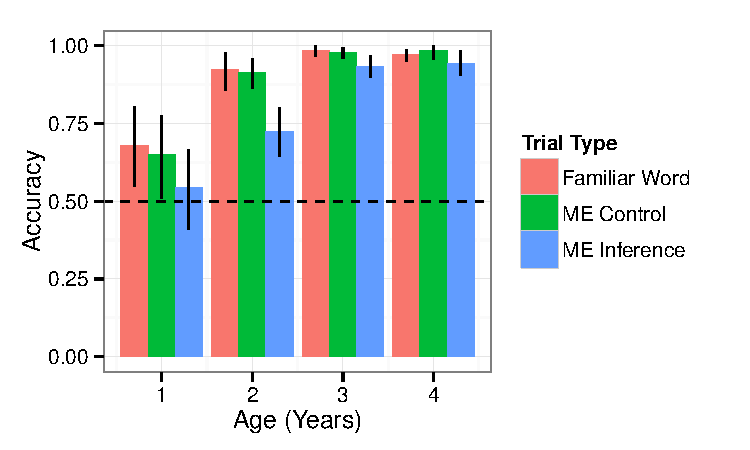
\includegraphics[width=5in]{figures/accuracy.pdf} 
    \caption{\label{fig:accuracy} Accuracy in our word recognition task, plotted by age group and trial type. Dashed line shows chance performance. Error bars show 95\% confidence intervals, computed by non-parametric bootstrap. }
  \end{center} 
\end{figure}

Accuracies for familiar word trials were above chance even for the one-year-old age group and rapidly approached ceiling performance in the two-year-olds (Figure \ref{fig:accuracy}). There were also no substantive differences in accuracy between Familiar Word and ME control trials. In contrast, ME Inference trials were substantially more difficult for children, with one-year-olds performing at chance, and two-year-olds showing a substantial decrement in performance for these trials.\footnote{To test the reliability of these differences, we fit a logistic mixed effects model to the data \cite{jaeger2008}; Our model specification included age group (coded as a discrete factor with one-year-olds as the intercept), trial type, and interactions of age group and trial type. Models with larger random effect structures did not converge, so we included only a random intercept for each participant. We found a significant increase in performance for all three older age groups ($\beta = 1.68,~3.21,~2.60$, all $p$s $< .0005$) and a significant decrement in performance for ME Inference trials  ($\beta = -1.14$, $p = .0003$), but no effect in ME Control trials and no interactions between trial type and age group (all $p$s $> .18$). 
%This model thus supports the findings of reliable developmental differences as well as a reliable decrement in performance for mutual exclusivity trials.
} 
Our data thus support the appropriateness of the tablet-based method for children two years old and above: These children were able to complete our task successfully and performed quite well, on average. As discussed below, accuracies for the one-year-olds (who were mostly above 18 months) were more mixed, but still had some within-subject reliability.

  %                                           Estimate Std. Error z value Pr(>|z|)    
% (Intercept)                                   1.1595     0.2990   3.878 0.000105 ***
% factor(age.group)2                            1.6828     0.4610   3.651 0.000262 ***
% factor(age.group)3                            3.2065     0.6790   4.722 2.34e-06 ***
% factor(age.group)4                            2.5992     0.5805   4.478 7.54e-06 ***
% trial.typeMEcontrol                          -0.4338     0.3259  -1.331 0.183114    
% trial.typeMEexperimental                     -1.1353     0.3191  -3.558 0.000374 ***
% factor(age.group)2:trial.typeMEcontrol        0.1232     0.5205   0.237 0.812910    
% factor(age.group)3:trial.typeMEcontrol        0.1449     0.8396   0.173 0.862955    
% factor(age.group)4:trial.typeMEcontrol        0.9881     0.8111   1.218 0.223091    
% factor(age.group)2:trial.typeMEexperimental  -0.6019     0.4752  -1.267 0.205244    
% factor(age.group)3:trial.typeMEexperimental  -0.4034     0.7262  -0.555 0.578583    
% factor(age.group)4:trial.typeMEexperimental   0.4269     0.6484   0.658 0.510337    



\begin{figure}[t] 
  \begin{center} 
    \includegraphics[width=5in]{figures/rt_dist.pdf} 
    \caption{\label{fig:rtdist} A histogram of reaction times across all participants. Red and blue curves show the best-fitting distributions found by a 2-component Gaussian mixture model, scaled for comparison to the histogram. Dashed lines show the cutoff values we adopted (.5 and 4.0 s).}
  \end{center} 
\end{figure}

We next turned to the reaction time data. Considering only reaction times for correct trials, we found a substantial skew in the reaction times we collected (Figure \ref{fig:rtdist}). This pattern appeared to be due to two clusters of reaction times: one larger, tighter cluster early on, representing immediate responding, and one broader slower cluster representing trials on which participants were unsure how to respond, looked to a parent, or otherwise deliberating. In an exploratory analysis, we fit a Gaussian mixture model (using the \texttt{mclust} package in \texttt{R}) and found that the best BIC values were indeed produced by a two-cluster solution, which is shown in Figure \ref{fig:rtdist}. 

For further analysis, we excluded reaction times faster than 500 ms or slower than 4000 ms. These values were determined post-hoc, based on visual inspection of the distribution. They correspond well both to our intuitions about the task and to the properties of the first mixture component found by the mixture model (for which mean + 3 standard deviations was 3928 ms). Excluding based on these threshold values resulted in a loss of 10.9\% of values.\footnote{Although this proportion seems high, consider the collection of reaction times based on eye-tracking methods. In these analyses, only half of trials are considered---those where the eyes are on the distractor item at the point of disambiguation \cite{fernald2008}.} In future work, we recommend the adoption of {\it a priori} standards for reaction time exclusion; we did not do so here because establishing such standards was a primary goal of the current experiment. 

\begin{figure}[t] 
  \begin{center} 
    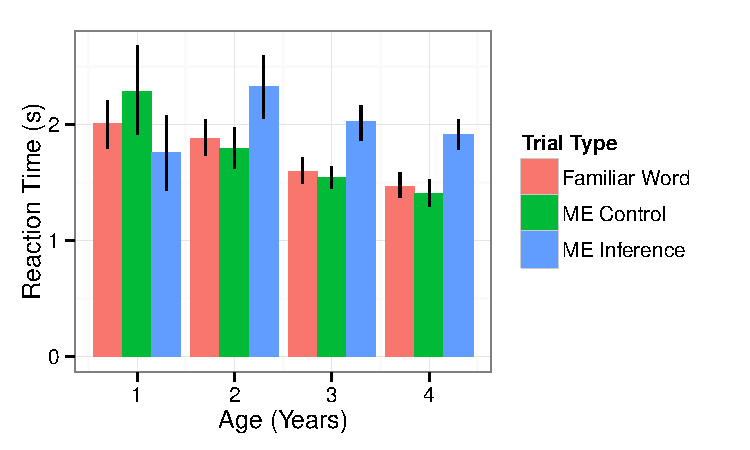
\includegraphics[width=5in]{figures/rt.pdf} 
    \caption{\label{fig:rt} Reaction times in our word recognition task, plotted by age group and trial type. Error bars show 95\% confidence intervals, computed by non-parametric bootstrap.}
  \end{center} 
\end{figure}

Older children were faster overall in our task, and ME inference trials were slower than both Familiar Word and ME Control trials for all groups except the one-year-olds (Figure \ref{fig:rt}). We again did not observe large numerical differences between Familiar Word and ME Control trials.\footnote{A linear mixed effects model fit to log-transformed reaction-time data showed a significant effect of trial number such that reaction times decrease over the course of the experiment ($\beta = .001$, $p = .04$), and three- and four-year-olds were significantly faster than one-year-olds ($\beta = -.19,~.26$, $p$s $<.005$). There were no main effects of trial type, but there were reliable slowdowns for ME Inference trials across the two-, three-, and four-year-olds ($\beta=.25,~.26,~.29$, all $p$s $< .0001$). ME control trials were also reliably faster for the four-year-olds ($\beta=-.13$, $p=.04$).} Experimenting with other reaction-time outlier exclusion processes did not qualitative alter the pattern of results. Nevertheless, we recommend that investigators using this method carefully examine their distribution of reaction times, as averages can be heavily skewed by just a small number of very long RTs.

% latex table generated in R 3.0.2 by xtable 1.7-3 package
% Fri Aug  1 11:05:54 2014
\begin{table}[t]
\centering
\caption{\label{tab:reliability} Mean reliability values found by a bootstrap sample of random splits of the data from familiar word trials. Values marked SB are computed by the Spearman-Brown prediction formula.}
\begin{tabular}{rcccc}
  \hline
Age group & Accuracy & Reaction time & Accuracy (SB) & Reaction time (SB) \\ 
  \hline
1-year-olds & 0.45 & 0.09 & 0.61 & 0.05 \\ 
2-year-olds & 0.31 & 0.34 & 0.42 & 0.44 \\ 
3-year-olds & -0.12 & 0.49 & -0.27 & 0.64 \\ 
4-year-olds & 0.03 & 0.60 & 0.03 & 0.74 \\ 
   \hline
\end{tabular}
\end{table}

Group-level developmental differences such as those described above do not necessarily signal a measure with high reliability. We computed split-half reliability coefficients for accuracy and reaction time based on splitting all trials using familiar words (both Familiar Word and ME Control trials) into two halves and computing the correlation between these two halves. To ensure the robustness of the statistic, we repeated this procedure with 1000 bootstrap replicates (different splits of the trials) and took the average value across these replicates. We also adjusted reliabilities using the Spearman-Brown prediction formula \cite{bartko1976} to estimate the overall reliability of the full sample of 16 items.

Reliabilities are shown in Table \ref{tab:reliability}. Accuracy and reaction time show opposite patterns: while accuracy was somewhat reliable for the youngest two age groups, the presence of a ceiling effect effectively eliminates any reliability for accuracies in the older two groups. In contrast, reaction times were not reliable for the one-year-olds but increased in reliability for the older age groups. These data thus suggest that even a sample of 16 trials can yield reliable data, especially for reaction times in the older age groups. In future work, a larger sample of trials (e.g. 32 familiar word trials) would even yield reliabilities above .65 for two-year-olds.

\section{Conclusions and Methodological Recommendations} 

We presented a simple method for creating tablet ``apps'' that allows experimenters to create basic websites and use these websites to collect data. This method is substantially easier and more flexible than platform-native app development, which can be costly and time-consuming. In addition, our method allows cross-platform compatibility and easy sharing for the resulting experiments. We showed in a simple word recognition experiment that this method yields reliable reaction time and accuracy data for children as young as two years old. Data collection using tablets thus has the potential to supplement and perhaps even supplant many behavioral methods currently in use. 

We summarize our methodological recommendations for the use of tablets:

\begin{enumerate}
\item Web-based experiment development can be a valuable tool for designing low-cost tablet experiments. This method should be considered for research applications that can be conducted in a setting with internet connectivity.
\item Tablets are a viable data collection even for very young children (potentially as young as 18 months), but if children have not interacted with a tablet before, care must be taken to familiarize children with the device prior to data collection. We used a simple ``dot game'' to practice the use of the tablet and found that this was partially effective in promoting more precise gestures.
\item Tablets can yield reliable and precise reaction time data, but care must be taken in the analysis to establish a priori procedures for the detection and removal of outliers; otherwise, analyses will be subject to post-hoc bias based on data cleaning choices. 
\end{enumerate}

Mobile and tablet-based computers are quickly becoming a ubiquitous part of life---and of childhood. Children play with their parents' and their own devices, and such devices are used for education, reading, games, and video chat with friends and relatives. Many important developmental issues are raised by this ubiquity, and more research must be done to determine how, when, and what children can learn from different kinds of devices. Nevertheless, the opportunity posed by such devices for developmental psychologists is immense.

\newpage

\bibliographystyle{apacite}
\bibliography{tablet}

\end{document}
